\documentclass[aps,%
12pt,%
final,%
oneside,
onecolumn,%
musixtex, %
superscriptaddress,%
centertags]{article} %%
\topmargin=-40pt
\textheight=650pt
\usepackage[english,russian]{babel}
\usepackage[utf8]{inputenc}
%всякие настройки по желанию%
\usepackage[colorlinks=true,linkcolor=blue,unicode=true]{hyperref}
\usepackage{euscript}
\usepackage{supertabular}
\usepackage[pdftex]{graphicx}
\usepackage{wrapfig}
\usepackage{subfigure}
\usepackage{amsthm, amssymb, amsmath}
\usepackage{textcomp}
\usepackage[noend]{algorithmic}
\usepackage[ruled]{algorithm}
\selectlanguage{russian}
%пользовательское
\DeclareMathOperator{\minimize}{minimize}
\DeclareMathOperator{\sign}{sign}
\DeclareMathOperator*{\argmin}{argmin}
\DeclareMathOperator*{\argmax}{argmax}

\begin{document}

\begin{titlepage}
\begin{center}
% Upper part of the page
\textbf{\large Санкт-Петербургский государственный университет} \\[0.8cm]
\textbf{\large Математико-механический факультет} \\[6.7cm]

% Title
\textbf{\LARGE Погорелов Петр Глебович}\\[1.0cm]
\textbf{\Large Лекционные материалы по теме <<Вероятностные алгоритмы тематического моделирования документов: Probabilistic Latent Semantic Analysis и Latent Dirichlet Allocation>>} \\[0.4cm]
\textbf{\Large Учебная дисциплина <<Теория Байесовский сетей>>} \\[5.7cm]

%supervisor
\begin{flushright} \large
\textbf{Руководитель:} \\
\textbf{д. ф.-м. н., профессор Тулупьев А.Л.}
\end{flushright}
\vfill

% Bottom of the page
{\large \textbf{{Санкт-Петербург}}} \par
{\large \textbf{{2018}}}
\end{center}
\end{titlepage}

\begin{titlepage}
\begin{center}
% Upper part of the page
\textbf{\Large SAINT PETERSBURG STATE UNIVERSITY} \\[0.6cm]
\textbf{\large Mathematics\&Mechanics Faculty} \\[6.7cm]

% Title
\textbf{\LARGE Pogorelov Petr}\\[1.0cm]
\textbf{\Large Lecture notes on <<Probabilistic algorithms of topic modelling: Probabilistic Latent Semantic Analysis and Latent Dirichlet Allocation>>} \\[0.4cm]
\textbf{\Large Theory of Bayesian Networks} \\[5.7cm]

%supervisor
\begin{flushright} \large
\textbf{Scientific supervisor:} \\
\textbf{Ph.D., Professor , Alexander Tulupyev}
\end{flushright}
\vfill

% Bottom of the page
{\large \textbf{{Saint Petersburg}}} \par
{\large \textbf{{2018}}}
\end{center}
\end{titlepage}

% Table of contents
\tableofcontents
\setcounter{page}{3}

\newpage
\section*{Введение}
\addcontentsline{toc}{section}{Введение}
\hspace{0.4cm}
Цель настоящей работы – введение в модели тематического моделирования для слушателей курса <<Теория байесовых сетей>>, которые раньше не сталкивались с данным классом методов. Для достижения этой цели были поставлены задачи:
\begin{enumerate}
  \item сформулировать постановку задачи тематического моделирования,
  \item дать описание алгоритма Probabilistic Latent Semantic Analysis, привести пример использования,
  \item дать описание алгоритма Latent Dirichlet Allocation, привести пример использования.
\end{enumerate}
Тематическое моделирование – одна из задач обработки естественных языков (NLP) без учителя, очень близкая к идее мягкой кластеризации. Большинство моделей тематического моделирования строятся на следующих предпосылках:
\begin{itemize}
\item каждый документ отписывается некоторым набором (смесью) тем;
\item каждая отдельная тема описывается некоторым набором токенов (слов).
\end{itemize}
\parТемы – это некоторые скрытые величины, которые присутствуют в наборе данных, но наблюдать их влияние напрямую – нельзя. Соответственно, задача тематического моделирования – извлечь эти скрытые величины и проанализировать их влияние на имеющийся набор данных.\parНа текущий момент, существует большое количество алгоритмов тематического моделирования. Важно отметить, что область их применения не ограничивается сферой NLP, они в той же степени эффективны и в задачах биоинформатики, физики и др. Однако наиболее популярны они, все таки, именно в задачах NLP.

\newpage
\section*{Модели тематического моделирования}
\addcontentsline{toc}{section}{Модели тематического моделирования}
\hspace{0.4cm}
Наиболее известный – латентный семантический анализ (или LSA). Данный метод идейно близок к методу главных компонент, который так же ищет скрытые величины (главные компоненты) в тексте. Однако, если в случае PCA решается задача поиска некоторой матрицы P, произведение матрицы факторов на которую порождает набор некоррелированных случайных величин меньшей размерности (как раз – скрытые величины).  То в случае LSA – раскладывается специальная матрица, построенная на основе TF-IDF статистики, рассчитываемой по корпусу документов. В обоих случаях на промежуточных этапах (диагонализация) используется алгоритм SVD .
\parАлгоритм PLSA представляет собой вероятностную версию алгоритма LSA, имеющую более интуитивную интерпретацию. Алгоритм LDA – представляет собой усовершенствованную версию PLSA алгоритма, который менее подвержен проблеме переобучения за счет уменьшения количества параметров в модели. Далее будет представлен разбор обоих методов вероятностного тематического моделирования.


\newpage
\section*{Модель PLSA}
\addcontentsline{toc}{section}{Модель PLSA}
\hspace{0.4cm}
Предположим, что имеется набор документов $d \in \mathcal{D}$, набор слов $w \in \mathcal{W}$ и набор тематик $z \in \mathcal{Z}$. Обозначим степень релевантности документа d топику z как $P(d\ |\ z)$. Данную величину можно трактовать как вероятность того, что документ d относится к топику z, либо сколько процентов содержания документа d относится к топику z. Аналогично, обозначим степень релевантности слова w топику z как $P(w\ |\ z)$. Данную величину можно трактовать как вероятность того, что слово w можно встретить в документах, которые полностью посвящены тематике z. Далее формализуем процесс генерации документа в контексте модели PLSA.\par
\begin{itemize}
\item выбираем документ $d \in \mathcal{D}$ с вероятностью $P(d)$,
\item генерируем слово $w_i$ для выбранного документа d по следующим правилам
    \begin{itemize} 
        \item выбираем тематику $z \thicksim P(z\ |\ d)$ – мульт-е р-е.
        \item выбираем слово $w \thicksim P(w\ |\ z)$ – мульт-е р-е.
     \end{itemize}
\end{itemize}
\parДалее опишем процесс оценки вероятностей $P(z\ |\ d)$ и $P(w\ |\ z)$. Предположим, что величины w и d условно независимы  относительно z [\ref{fig:plsa}].
\begin{figure}[h!]
  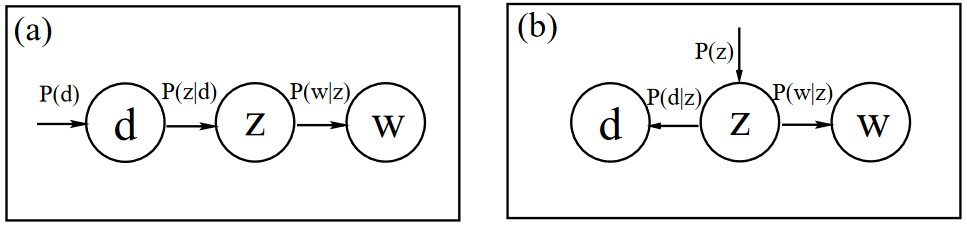
\includegraphics[width=\linewidth]{PLSA_graph.jpg}
  \caption{Эквивалентные графические модели параметризации совместного распределения пары  (w,d) с учетом новой скрытой величиной z \cite{hoffman1}.}
  \label{fig:plsa}
\end{figure}
\parВероятность наблюдения пары (w,d) можно выразить следующим образом: $P(w, d)=P(d)P(w\ |\ d)$, или, что эквивалентно (помним об условной независимости случайных величин w и d относительно z)
$$P(d, w) = P(w, d) = \sum_{z}^{\mathcal{Z}} P(z)P(w\ |\ z)P(d\ |\ z)$$
Данное выражение полностью эквивалентно следующему
$$P(d, w) = \sum_{z}^{\mathcal{Z}} \dfrac{P(z)P(w\ |\ z)P(d)P(z\ |\ d)}{P(z)}=P(d)\sum_{z}^{\mathcal{Z}} P(w\ |\ z)P(z\ |\ d)$$
\parТаким образом, была формализована модель порождения документов для PLSA. Оценить её неизвестные параметры можно с помощью алгоритма оценки максимального правдоподобия. В выражении фигурирует функция $q(w,\ d)$, которая оценивает, сколько раз некоторый символ встретился в документе. $q(d)$ – выражает длину документа в словах. Построим функцию правдоподобия.
$$L = \prod_{w}^{\mathcal{W}}\prod_{d}^{\mathcal{D}} P(d, w)^{q(w, d)} = \prod_{w}^{\mathcal{W}}\prod_{d}^{\mathcal{D}}\bigg(P(d)\sum_{z}^{\mathcal{Z}} P(w\ |\ z)P(z\ |\ d)\bigg)^{q(w, d)},$$
$$\log L = \sum_{w}^{\mathcal{W}}\sum_{d}^{\mathcal{D}}q(w, d)\bigg(\log P(d) + \log\sum_{z}^{\mathcal{Z}} P(w\ |\ z)P(z\ |\ d) \bigg)=$$
$$\sum_{d}^{\mathcal{D}}q(d)\Bigg(\log P(d) + \sum_{w}^{\mathcal{W}}\frac{q(w, d)}{q(w)}\bigg(\log\sum_{z}^{\mathcal{Z}} P(w\ |\ z)P(z\ |\ d)\bigg)\Bigg)$$
\parТеперь необходимо некоторым образом максимизировать лог - правдоподобие по параметрам $P(w\ |\ z)$, $P(z\ |\ d)$: $$p^*(z\ |\ d), p^*(w\ |\ z) = \argmax_{P(z\ |\ d),\ P(w\ |\ z)} log L$$ 
\parВеличина $P(d)$ никак не влияет на оптимизацию, поскольку постоянна для данного набора документов, и в случае, если все документы в выборке уникальны, выражается как $P(d)=\frac{1}{(|D|)}$.  Авторы оригинальной статьи предлагают использовать для оценки неизвестных параметров EM – алгоритм. Подробно с данным алгоритмом и его применением к текущей задаче можно ознакомиться в \cite{hoffman1}. Помимо этого, был подготовлен блокнот Jupyter с иллюстрацией механизма работы данного алгоритма. Блокнот предоставляется в комплекте с лекционными материалами.

\parДалее будет рассмотрен пример использования PLSA на наборе данных “20 Newsgroup Dataset” . Это один из наиболее популярных наборов данных для тестирования различных NLP моделей. Он состоит из 20 тысяч документов, каждый из которых посвящен одной из 20 тематик и содержит текст дискуссии на специализированном форуме.
\parРассмотрим наиболее релевантные слова для каждой категории. Для этого необходимо отсортировать слова по вероятностям для первой категории $P(w\ |\ z=0)$ и второй категории $P(w\ |\  z=1)$ в порядке возрастания. В рамках данной задачи выборка была ограничена двумя тематиками. Первая – специализированный форум по программированию в среде Windows, вторая – религиозный форум. Всего в наборе 1192 документов, словарь ограничен 1000 наиболее часто встречающимися словами (за исключением общих стоп-слов английского языка).

\newpage
\parПо ключевым ключевым первой тематики [\ref{fig:plsa_demo}] (\textit{god, will, people, jesus}) легко заметить, что все они относятся к религиозной теме. Ключевые слова второй тематики (\textit{com, windows, file}) имеют непосредственное отношение к вычислительным системам.

\begin{figure}[h!]
  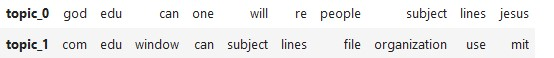
\includegraphics[width=\linewidth]{PLSA_demo.jpg}
  \caption{Наиболее часто встречающиеся слова в двух тематиках, выделенных алгоритмом PLSA.}
  \label{fig:plsa_demo}
\end{figure}

\newpage
\section*{Модель LDA}
\addcontentsline{toc}{section}{Модель LDA}
\hspace{0.4cm}
Модель Latent Dirichlet Allocation, предложенная Blei D., Ng A., Jordan M. [\cite{andrewng1}] решает ту же самую задачу, что и PLSA, но исходит из других предпосылок о процессе порождения документов. Авторы статьи отмечают, что PLSA имеет серьезный недостаток: необходимость расчета оценок $|Z|*(|D|\ +\ |W|)$ параметров мультиномиальных распределений (де-факто мультинулли). Легко заметить, что это число линейно возрастает с увеличением документов в обучающей выборке. Таким образом, модель PLSA может быть подвержена оверфиттингу. Авторы предлагают подход, позволяющий устранить зависимость числа параметров от объема корпуса документов.
Формализуем процесс генерации документа моделью LDA [\ref{fig:lda}]:
\begin{figure}[h]
  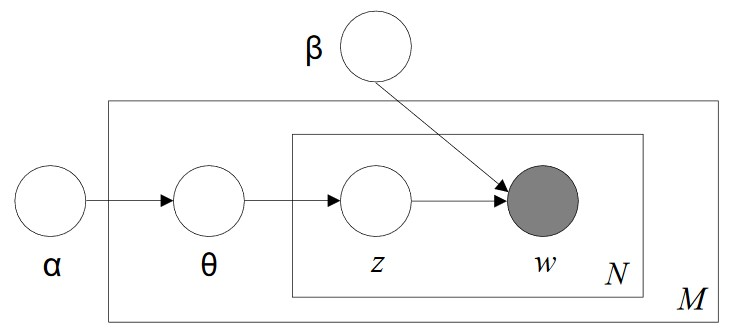
\includegraphics[width=\linewidth]{LDA_graph.jpg}
  \caption{Графическое представление модели LDA}
  \label{fig:lda}
\end{figure}

\begin{itemize}
    \itemвыбираем длину документа N (авторы предлагают генерировать $N \thicksim Poisson(\xi)$),
    \itemгенерируем вектор вероятностей $\theta \thicksim Dir(\alpha)$,
    \itemгенерируем слова для документа длины N:
    \begin{itemize}
        \itemвыбираем тематику $z_i  \thicksim Multinomial(\theta)$,
        \itemвыбираем слово $w_i  \thicksim Multinomial(\beta_{z_i})$.
    \end{itemize}
\end{itemize}
\parВ данном случае вектор $\theta$, полученный путем семплирования из распределения Дирихле  с параметром $\alpha$ представляет собой долю, на которую тематика  z представлена в тексте. Вектор $\beta_{z_i}$  (строка матрицы $\beta$) представляет собой относительную важность слов в тематике $z_i$ (вероятность встретить слово в данной тематике).  Распределение Дирихле в данном случае выступает в роли сопряженного априорного распределения  для z, поскольку его очень удобно использовать при переоценивании параметров мультиномиального распределения.

\parОценка коэффициентов модели LDA сводится к оценке параметров $\alpha$ и $\beta$. Авторы работы предлагают использовать для этого алгоритм \textbf{<<Variational Bayes>>}. С работой данного алгоритма можно ознакомиться в оригинальной статье.
\parДалее к рассмотрению предлагается пример использования модели LDA на наборе данных “20 Newsgroup Dataset”. Для чистоты эксперимента выборка была ограничена двумя тематиками, как и в примере использования PLSA. Первая – специализированный форум по программированию в среде Windows, вторая – религиозный форум. Точно так же используется 1000 наиболее часто встречаемых слов из набора 1192 документов. [\ref{fig:lda_demo}]
\parЛегко заметить, что алгоритм LDA выделил те же самые слова, что и PLSA, но придал им другой уровень значимости. В частности, слово “jesus” в религиозной тематике алгоритма LDA имеет больший вес, нежели тот, что ей придал алгоритм PLSA.

\begin{figure}[!h]
  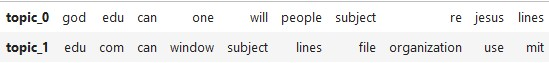
\includegraphics[width=\linewidth]{LDA_demo.jpg}
  \caption{Наиболее часто встречающиеся слова в двух тематиках, выделенных алгоритмом LDA}
  \label{fig:lda_demo}
\end{figure}

\newpage
\section*{Заключение}
\addcontentsline{toc}{section}{Заключение}
\hspace{0.4cm}
В рамках настоящей работы было сформулировано понятие тематического моделирования, обозначены предпосылки, на которых базируются алгоритмы решающие данный класс задач. Было произведено подробное описание и примеры использования модели Probabilistic Latent Semantic Analysis, на базе которой строится большинство алгоритмов тематического моделирования. В т.ч. Latent Dirichlet Allocation, Additive Regularization Topic Modelling [\cite{vorontsov1}]. Также была кратко рассмотрена модель LDA и приведен пример ее использования для задачи выделения тематик в корпусе документов.

%автоматическая генерация библиографии из бибтеховского файла. Из файла подгрузятся только те статьи, на которые есть ссылки в тексте!
\bibliographystyle{utf8gost705u}
\bibliography{biblio}
\end{document}


